\documentclass[12pt]{article} 
\usepackage{amsmath} 
\usepackage[dvips]{graphicx}
\usepackage{multirow} 
\usepackage{geometry} 
\usepackage{pdflscape}
\usepackage[labelfont=bf]{caption} 
\usepackage{setspace}
\usepackage[running]{lineno} 
% \usepackage[numbers,sort]{natbib}
\usepackage[round]{natbib} 
\usepackage{array}
\usepackage[table]{xcolor}
\usepackage{xr}

\newcommand{\methods}{\textit{Materials \& Methods}}
\setcounter{section}{0}
\renewcommand{\thesection}{S\arabic{section}}
\setcounter{table}{0}
\renewcommand{\thetable}{S\arabic{table}}%
\setcounter{figure}{0}
\renewcommand{\thefigure}{S\arabic{figure}}%
\setcounter{equation}{0}
\renewcommand{\theequation}{S\arabic{equation}}
\renewcommand{\labelenumi}{S\arabic{enumi}}


\topmargin -1.5cm % 0.0cm 
\oddsidemargin 0.0cm % 0.2cm 
\textwidth 6.5in
\textheight 9.0in % 21cm
\footskip 1.0cm % 1.0cm

\usepackage{authblk}

\begin{document} 

\title{Motif roles provides unique information about species risk of extinction\\ \medskip Supplementary Information}


\author{Anna \r{A}kesson$^{1\dagger}$, Alyssa R. Cirtwill$^{2}$, Kate L. Wootton$^{3}$, Anna Ekl\"{o}f$^{1}$} 
\date{\small$^1$Department of Theoretical Biology, Chemistry, and Physics\\ 
Link\"{o}ping University\\
Link\"{o}ping, Sweden\\
\medskip
\small$^2$Department of Agricultural Sciences\\
University of Helsinki\\
Helsinki, Finland\\
\medskip
\small$^3$ BioFrontiers Institute\\
University of Colorado, Boulder\\
U.S.A.
\medskip
$^\dagger$ Corresponding author:\\
}



\maketitle 
\raggedright

\setlength{\parindent}{15pt} 
\begin{spacing}{2.0}

\clearpage

\section*{Table of contents}
    \begin{spacing}{1.0}

    Appendices S1-S3 provide supplemental methods, while appendices S4-S8 provide supplemental results.

    \begin{enumerate}
    
        \item Calculating persistence

            \begin{itemize}
                \item Details on functional response of consumers
                \item Contains Eqn. S1
            \end{itemize}    
            

        \item Network creation \\
        
            \begin{itemize}
            \item Construction of simulated networks
            \item Filtering of biologically unrealistic networks 
            \item Conversion of networks to acyclic form
            \item Comparison of empirical and simulated networks
            \end{itemize}
            
            
        \item Statistical analysis

            \begin{itemize}
                \item Species persistence and motif participation (Eqn. S2-3)
                \item Motif participation and network properties (Eqn. S4-6)
                \item Network mean persistence and motif profiles (Eqn. S7)
                \item Network motif profiles and global network structure (Eqn. S8)
                \item Persistence and other network properties (Eqn. S9-11)
            \end{itemize}
                

        \item Persistence and motif participation
            \begin{itemize}
                \item Contains Table S1
            \end{itemize}


        \item Participation and network properties

            \begin{itemize}
                \item Contains Table S2
                \item Contains Fig. S1
            \end{itemize}
    
        \item Persistence, degree, and trophic level

            \begin{itemize}
                \item Contains Table S3
                \item Contains Fig. S2-3
            \end{itemize}    

        \item Within-network motif-persistence relationships

            \begin{itemize}
                \item Contains Fig. S4
            \end{itemize}    
    
        \item Persistence and network motif profiles

            \begin{itemize}
                \item Contains Table S4
            \end{itemize}   
        
        \item Motif profiles and global properties

            \begin{itemize}
                \item Contains Figure S5
                \item Contains Table S5
            \end{itemize}

        \item Persistence and global network properties
            \begin{itemize}
                \item Contains Figures S6, S7
                \item Contains Table S6
            \end{itemize}

        \item Glossary    

            \begin{itemize}
                \item Contains Table S7
            \end{itemize}


    \end{enumerate}    
\end{spacing}
\clearpage

\linenumbers
\section{Calculating persistence}        

        We use Bayesian network modelling to calculate the persistence of each species in our simulated networks. 
        A Bayesian network represents a graphical model for probabilistic relationships among a set of variables. 
        In our ecological setting, the nodes of the network represent species and links represent feeding interactions between species.
        In network-theory terms, the species are Bernoulli random variables, and the links represent conditional dependencies among these variables. 
        Each node has a set of local probability dependencies, conditional on the state of the parent nodes. 
        Since the nodes are species, their state can be either extant or extinct.
        The extinction probability of each species is a function of the state of its resources and also depends on a baseline probability of extinction ($\pi$) representing risk of extinction due to factors unrelated to network structure.
        In our baseline scenario, basal resources had a baseline extinction probability of $\pi = 0.1$. 
        We also simulated a set of scenarios where basal resources had a higher baseline probability of extinction ($\pi$). 
        These scenarios reflect threats to basal resources such as increased temperatures resulting in droughts, making some species more vulnerable to extinction.
        $\pi$ ranged between $0.1-0.5$, in steps of $0.08$. 
        The highest disturbance level, $\pi = 0.5$, corresponds to basal species having a 50\% risk of going extinct. 
        Consumer species retained $\pi=0.1$ in all cases.


    \subsection{Functional response of consumers}

        The response of a consumer to the loss of a fraction of its resources can be modelled in several biologically plausible ways: i) a topological response, where the consumer's probability of extinction is constant unless all resources are lost, ii) a linear response, in which the extinction probability increases linearly with resources loss, and iii) several nonlinear responses where the probability of extinction increases non-linearly with the fraction resource lost. 
        The extinction probability will differ depending on the response function.
        
        
        A sigmoid non-linear functional response of consumers to the loss of resources ($\alpha >1, \beta >1$) has been shown to most accurately capture the secondary extinctions produced by a dynamical model~\citep{Eklof2013}.
        Therefore, we use a cumulative density function of a beta distribution to get each species \textit{i} probability of extinction:
        \begin{equation}
        \label{betafunc}
        P(\lnot i|f) = \pi + (1 - \pi) \frac{B(f;\alpha,\beta)}{B(\alpha,\beta)}
        \end{equation}
        

        \noindent If all resource species of a consumer \textit{C} are present ($f = 0$), the extinction probability will be $P(\lnot C|f) = \pi$. 
        Similarly, if all resources are extinct ($f = 1$), the extinction probability $P(\lnot C|f)$ will be equal to 1 and the consumer will go extinct.
        If the fraction $f$ is not 1 nor 0, the non-linear sigmoid curve will determine the response of the consumer, which will be more severe if the fraction resources lost is high and less severe if the fraction is small. This will in turn affect the extinction probability $P(\lnot C|f)$. 
        For a basal species, we assume that abiotic resources are always available. Therefore, a primary producer is independent of resource species and will always have $f = 0$.  
        

        As consumer species depend on their resources, we start by determining the status of each primary producer in the network.
        Systematically, we use Equation \ref{betafunc} to calculate each species' probability of extinction $P(\lnot i|f)$, and then perform Bernoulli trials to determine whether the species goes extinct or not. 
        Imagine a basal species \textit{A} with extinction probability $P(\lnot A) = \pi$ where $\pi = 0.1$. We draw a random number $r$ from a uniform distribution between $0-1$. The basal species would be considered extinct if $r < 0.1$, and extant otherwise. 
        
        
        We then insert the simulated fraction of species lost into Equation \ref{betafunc} to calculate $P(\lnot C|f)$ for the consumer species \textit{C}. 
        In the same manner as for the basal species above, we compare $P(\lnot C|f)$ with a random number $r$, and if $r < P(\lnot C|f)$ the consumer species is considered extinct. 
        In this way, we evaluate each species existence, starting from the bottom and working our way up.
        
        
        As this method is probabilistic, we repeat these calculations 100 000 times per network, with unique random draws.
        For each species, we then estimate the fraction of simulations in which the species persist, and this value is the approximated probability of persistence.
        To approximate persistence probabilities through numerical simulation are shown to be highly efficient and produce the same result as exact methods of solving Bayesian networks \citep{Haussler2020}.
        
        
\clearpage


\section{Network creation}

    \subsection*{Generation of simulated networks}

        We simulated a suite of food webs based on the probabilistic niche model, which assigns predator-prey links based on the body-mass ratios between individuals of different species~\citep{Williams2000,Delmas2017}. The meso-scale structure of niche-model networks closely mimics that of empirical food webs~\citep{Stouffer2007}. To ensure that we captured a variety of realistic community sizes and structures, we generated networks ranging between 50 and 100 species (in steps of 10) with connectance values between 0.02 and 0.2 (in steps of 0.02). The range of network sizes was chosen to reflect moderately well-sampled empirical webs while working within our computational limits, while the range of connectance values was chosen to cover that observed in most empirical food webs~\citep{Dunne2002e}. We generated a total of 100 networks with each combination of parameters, for a total of 6000 networks. All networks were generated using the function "nichemodel" within the Julia language package \emph{BioEnergeticFoodWebs}~\citep{bioenergeticfw,Delmas2017}. If a simulated network contained any disconnected species (species without predators or prey) or disconnected components (a group of species connected among themselves but not to the rest of the network), the network was rejected and a new network simulated. Finally, networks where the path lengths between each species and a basal resource could not be resolved (i.e., trophic levels were undefined) were rejected and new networks simulated.


        After generating the network structure, we simulated community dynamics using the function ``simulate'' from the Julia language package \emph{BioEnergeticFoodWebs}~\citep{bioenergeticfw,Delmas2017}. This function uses Lotka-Volterra predator-prey models including density dependence and type 2 functional responses for all species (please see~\citet{Delmas2017} for full details).
        All non-basal species were designated as vertebrates to ensure a good match between metabolic and predator-prey body-mass ratio values. Metabolic rates in the Lotka-Volterra model are based on each species' body mass (i.e. mass of a single individual). We assigned relative body masses based on each species' trophic level, which was, in turn, calculated based on the food-web structure provided by the niche model. After basal species were assigned a body mass of 1, we used a predator-prey body-mass ratio of 3.065 to calculate the relative body masses of higher trophic levels. We selected this ratio based on the estimate for vertebrates (averaged across ecosystem and metabolic types) in~\citet{Brose2006}. We excluded reported body-mass ratios for invertebrates as these could include parasites and parasitoids, which are generally smaller than their prey, and because interactions among vertebrates are better represented in the food-web literature than interactions involving invertebrates.
        
        
        The persistence of each species in our simulated networks also depends on its population biomass. 
        We randomly assigned initial population biomasses (i.e. cumulative biomass across all individuals of a species) for each species from a uniform distribution [0,1]. Note that population biomasses and individual body masses are not calculated on the same scale. We then simulated community dynamics for 1000 time steps to obtain an `equilibrium' community. To ensure that species did not `recover' from unrealistically low biomasses during the simulation, we considered a species extinct if it dropped below an arbitrary threshold biomass of 1$\times10^{-5}$. When simulating initial (i.e. pre-disturbance or equilibrium) dynamics, we rejected any network where one or more species dropped below this biomass threshold. Consumers were assumed to have no preferences such that the consumption rate $w_{ij}$ of predator $i$ eating prey $j$ is equal to $\frac{1}{n}$, where $n$ is the number of prey for predator $i$. If the network did not retain all species for 1000 time steps, a new set of initial population biomasses was applied and the simulation repeated.
        If a set of biomasses where all species persist still had not been reached after 100 sets of randomly-assigned initial biomasses, we discarded the network and simulated another to replace it.
        
    
    \subsection*{Filtering of biologically unrealistic networks}

        After simulating our initial niche-model networks, we filtered networks for biological plausibility.
        Specifically, we removed any network containing disconnected components
        (species or groups of species not connected to the rest of the network) 
        or any network where any species had a shortest trophic level \textgreater6 as such high trophic levels are very uncommon in empirical food webs ~\citep{Riede2011}.
        Any removed network was replaced with a fresh simulation and re-checked until 100 realistic networks for each size-connectance combination had been obtained.
    

    \subsection*{Conversion of networks to acyclic form}

        A Bayesian food web depicts probabilistic relationships among a set of species where each species' probability of persistence depends upon the probabilities of its resource species persisting~\citep{Jensen_Nielsen,Eklof2013}. 
        All persistence calculations therefore begin by determining the status of the basal resources (who do not depend on other species).
        Calculations continue in a strictly bottom-up manner with primary consumers (who depend only on basal resources), and so on up the network.

            
        While niche-model food webs can contain cycles (e.g., species A eats B, B eats C, and C eats A), such cycles make it impossible to calculate persistence in the Bayesian network framework~\citep{Tarjan1972}. 
        We therefore removed any cycles within each network by removing the link in each cycle which contributed least to the robustness of the food web, following~\citet{Allesina2009functional}.
        This is achieved by first finding the set of resources for each consumer and then removing the consumer-resource connections which have the lowest eigenvalue centrality~\citep{Allesina2009functional}.
        These links have the least effect on the overall stability of the network; removing them creates an acyclic network with very similar properties to the original network.
        Next, we ordered the species from lowest to highest trophic level using a topological sorting routine following \citet{Tarjan1972} and \citet{Allesinaetal2005}, ensuring that probability calculations follow a strict bottom-up order. 
        After these steps, calculations of persistence probabilities can begin.
        

    \subsection*{Comparison of empirical and simulated networks}
    
    
        Although previous work has shown that the niche model replicates the motif structure of empirical networks~\citep{Stouffer2005a,Stouffer2006}, we provide a comparison of the motif profiles and consumer motif participation for our simulated networks and the highest-quality empirical networks we could find within the same size range.
        For this comparison, we obtained all networks containing 50-100 species from \citet{globalwebdb}.
        These webs ranged in connectance from 0.024-0.089
        We then removed networks where sets of predators and prey were completely different (i.e., bipartite networks) or links were not clear (i.e., +/- effects rather than predation specifically).
        This yielded five vertebrate-dominated food webs describing the California coast in different years, four invertebrate-dominated food webs describing mainland US streams, 23 invertebrate-dominated food webs describing New Zealand streams, and five other invertebrate-dominated food webs.
        This final set of webs had 50-77 species and connectances of 0.2-0.21 - the upper range of connectance in our simulations.
        This may be partly due to relatively poor resolution of basal resources in these empirical webs: aggregation of many taxa into nodes such as `phytoplankton' will tend to decrease the number of species but leave the number of links unchanged, raising connectance.
        We note that most of these webs were compiled by just three research groups.
        Moreover, many of the webs are repeated samples of the same site  or closely-grouped sites.
        This means that these empirical networks cannot be considered fully independent samples.
        
        
        \begin{figure}
            \includegraphics[width=\textwidth]{figures/motif_profiles_participation_vs_empirical.eps}
            \caption{\textbf{A)} Proportions of acyclic motifs in the motif profiles of empirical and simulated networks. Mean proportions ($\pm$SD) in the simulated networks are indicated in black, with the range of proportions in the simulated networks indicated by black boxes. \textbf{B)} Proportions of acyclic motifs in the motif participation vectors of consumers in simulated and empirical networks.}
            \label{empirical_compare}
        \end{figure}
        
    \subsubsection*{Comparing motif profiles}
    
      The proportions of omnivory and apparent competition in the motif profiles of simulated networks matched those of the empirical webs fairly well, but many of the empirical webs had higher proportions of direct competition and lower proportions of the three-species chain than any simulated web.
      The empirical webs with high proportions of direct competition tend to be invertebrate-dominated webs representing small streams.
      High proportions of direct competition in these system suggest large numbers of fairly generalist herbivore/detritivores, with relatively few secondary consumers present to create chains.
    
    
      A few webs had lower proportions of apparent competition than any simulated web but similar proportions of the other motifs.
      Most of these webs represented the California coast in different years (2003-2007).
      Basal resources in these webs were highly aggregated into only two size classes of phytoplankton and three types of detritus.
      This aggregation at the basal level leads to artificial ``specialisation'' in consumers with low trophic levels who may consume, for example, many species of phytoplankton that are grouped into a single size class.
      As the basal resources in our simulated networks are not aggregated, our webs feature higher proportions of apparent competition as seen in the other empirical webs.
    
    
    \subsubsection*{Comparing motif participation}
      
      Despite the differences in network motif profiles between some of the empirical food webs and the simulated webs, we note that the motif participation of consumers in the simulated webs entirely spans the range of motif participation for consumers in the empirical webs.
      Consumers in the NZ stream food webs had higher proportions of direct competition and lower proportions of apparent competition than the mean of the simulated webs, consistent with the network motif profiles.
      Nonetheless, the greater differences in network profiles than consumer motif participation suggests that the largest differences between the simulated and empirical networks are in the roles of basal resources.
      In empirical webs, basal resources are often highly aggregated. 
      Improved resolution at the basal level should improve the correspondence between simulated and empirical webs and allow better modelling of empirical communities.
    

\clearpage        

        
\section{Statistical analysis}

    \subsection{How does species persistence vary with motif participation?}

        We are first interested in whether participating more often in a certain motif (e.g., direct competition) might increase a species' probability of persistence.
        To test this, we fit four linear mixed-effect models (LMMs; one per motif included in the Bayesian networks):

        \begin{equation}
            \Psi_{ink} \approx \rho_{i} + \pi_{k} + \rho_{i}\pi_{k} +
            S_{n}:C_{n} + N_n,
            \label{propreq}
        \end{equation}


        \noindent where $\Psi_{ink}$ is the persistence of species $i$, belonging to network $n$, during disturbance level $k$, $\rho_{i}$ is the proportion of the role of species $i$ that is made up by the focal motif, $\pi_{k}$ is the probability of extinction for a basal resource in disturbance level $k$, and $S_{n}C_{n}$ is a random intercept for the species richness and connectance of the network containing species $i$, and $N_n$ is a random effect of network ID.
        The network-level random effect accounts for the fact that species in the same network are not independent.
        We centered and scaled the predictors before fitting the LMMs.
        All models were fit using the R~\citep{R} function `lmer' from the package \emph{lmerTest}~\citep{lmerTest}.
        We calculated marginal (fixed effects only) and conditional (fixed and random effects) $R^2$ using the R~\citep{R} function `r.squaredGLMM' from the package \emph{MuMIn}~\citep{MuMIn}.

        
        We were also interested in whether these general trends were consistent across networks with different global properties and different levels of disturbance. 
        To test this, we performed a linear regression of persistence against motif participation within each simulated network, for each level of disturbance to basal resources:

        \begin{equation}
            \Psi_{ik} \approx \rho_{i} ,
            \label{mineq}
        \end{equation}

        \noindent where all symbols are as in equation~\ref{propreq}.
        These regressions were fit using the R~\citep{R} base function `lm'.
        We then visually examine the distribution of slopes for the effect of motif participation across levels of disturbance, network size, and connectance. 


    \subsection{How does motif participation vary with network properties?}

        Species' motif participation may covary with other measures of network structure and species' roles within the network.
        To determine the relationships between motif participation and global network structure, we fit a set of four linear mixed-effect models (one per motif):

        \begin{equation}
            \rho_{in} \approx \Sigma_{n} + \zeta_{n} + \Sigma_{n}\zeta_{n} + N_n ,
            \label{partic_SC}
        \end{equation}
        
        \noindent where $\rho_{in}$ is the proportion of the role of species $i$, belonging to network $n$, that is made up by the focal motif,
        $\Sigma_{n}$ is the size of network $n$, $\zeta_{n}$ is the connectance of the network $n$, and $N_n$ is a random effect of network ID.
        Predictors were not centered or scaled before fitting.
        All models were fit using the R~\citep{R} base function `lm'.

       
        We fit a similar set of eight linear mixed-effect models relating motif participation to in-degree or trophic level:
        
        \begin{equation}
            \rho_{in} \approx \delta_{i} + S_{n}C_{n} + N_n,
            \label{partic_deg}
        \end{equation}

        \begin{equation}
            \rho_{in} \approx \tau_{i} + S_{n}C_{n} + N_n,
            \label{partic_tl}
        \end{equation}
        
        \noindent where $\rho_{in}$ is the frequency with which species $i$, belonging to network $n$, participates in the focal motif, $\delta_{i}$ is the in-degree of species $i$, $\tau_{i}$ is the shortest trophic level of species $i$, $S_{n}C_{n}$ is a random effect of the combination of size and connectance for network $n$, and $N_n$ is a random effect of network ID.
        These models were fit using the R~\citep{R} function `lmer' from the package \emph{lmerTest}~\citep{lmerTest}.

    		
    \subsection{How does mean persistence vary with motif profiles?}

        To test whether networks with similar motif profiles tend to have similar mean persistences among consumers, we fit a PERMANOVA relating Bray-Curtis dissimilarity in motif profiles to the mean persistence of all consumers in a network (averaged across all levels of disturbance to basal resources).
        As with the PERMANOVA relating motif participation to network properties, we fit the PERMANOVA using the R~\citep{R} function `adonis' from the package \emph{vegan}~\citep{vegan} and calculated significance based on 9999 permutations.


        We then tested whether dispersion was homogeneous across levels of persistence using an ANOVA and whether there was a linear relationship between persistence (rounded to three decimal places) and variability of motif profiles using a linear regression.
        Dispersion was calculated using the R~\citep{R} function `betadisper' from the package \emph{vegan}~\citep{vegan}.
        In case high or low mean persistence is associated with more variable network structure, we calculated dispersion of motif structure for each level of mean persistence (rounded to three decimal places to allow multiple networks to have the same value of mean consumer persistence and treated as a categorical variable). 

        
        To supplement these overall tests, we also fit four linear models relating mean persistence to network motif profiles, disturbance, and the interaction between them:

            \begin{equation}
                \overline{\Psi_{nk}} \approx \Bar{\rho}_{n} + \pi_{k} + \Bar{\rho}_{n}\pi_{k} ,
                \label{netpropeq}
            \end{equation}
        
        \noindent where $\overline{\Psi_{nk}}$ is the mean persistence of all consumers in web $n$ at disturbance level $k$, $\Bar{\rho}_{n}$ is the proportion of the focal motif in the network's motif profile, and $\pi_k$ is the level of disturbance (probability of extinction for basal resources) as in equation~\ref{propreq}. 
        All regressions were fit using the R~\citep{R} base function `lm'.
    

    \subsection{How do network motif profiles vary with global structure?}
    
        As well as affecting persistence directly, global network structure (i.e., size and connectance) may affect the meso-scale structure of the network.
        This is especially likely since we include only networks which can retain all initial species after 1000 rounds of simulated Lotka-Volterra population dynamics~\citep{Cirtwill2021_inprep}:  some meso-scale structures might be more likely to allow all species to persist than others in networks with different size and connectance constraints.
        We test whether networks with the the same size and connectance have more similar motif profiles using a PERMANOVA~\citep{Anderson2001} of Bray-Curtis dissimilarity among motif profiles against network size, connectance, and their interaction.
        Significance was calculated based on 9999 permutations.
        PERMANOVA tests may give false positive results if variability is not homogeneous among groups (i.e., levels of network size or connectance).
        To test whether this applies in our case, we fit an ANOVA of the dispersion of motif profiles about the centroid for each combination of network size and connectance. 
        We fit the PERMANOVA using the function `adonis', calculated dispersion using the function `betadisper', and fit the ANOVA using the function `anova', all from the R~\citep{R} package \emph{vegan}~\citep{vegan}.


        To gain a more detailed picture of how the proportion of each motif may vary with global network structure, we also fit four regressions (one per motif) relating the proportion of a motif in a network's motif profile to network size, connectance, and their interaction:

        \begin{equation}
            \Bar{\rho_{n}} \approx \Sigma_{n} + \zeta_{n} + \Sigma_{n}\zeta_{n}
        \end{equation}
        where all symbols are as in equations~\ref{propreq} and~\ref{netpropeq}.
        We fit each regression using the R~\citep{R} base function `lm'.
            

    \subsection{How does persistence vary with other properties?}

        \subsubsection{Network mean persistence and network properties}
    
            Both species richness (S) and connectance (C) are known to influence persistence in both simulation studies and empirical food webs.
            In addition, increasing the probability of extinction for basal species ($\pi$) is intended to decrease persistence of species at higher trophic levels.
            Although these effects are not the main focus of our manuscript, we must establish these background effects before measuring the effects of meso-scale structure on persistence.
            The persistence of basal species in our simulations is determined only by their baseline probability, being either $\pi = 0.1$ or higher, dependent on $\pi$.
            We therefore considered only non-basal species (i.e., those with at least one prey) throughout this manuscript.

            To test for effects of global network properties, we fit a linear regression relating the mean of consumer species' probabilities of persistence in a network to network size, connectance, the level of disturbance to basal resources, and all interactions between them. 
            All predictors were centered and scaled before fitting the model. 
            As the three-way interaction was significant, we did not simplify the model.
            All models were fit using the R~\citep{R} base function `lm'.


            \begin{equation}
                \overline{\Psi_{nk}} \approx \Sigma_{n} + \zeta_{n} + \pi_k + \Sigma_{n}:\zeta_{n} + \Sigma_{n}\pi_k + \zeta_{n}\pi_k + \Sigma_{n}\zeta_{n}\pi_k,
                \label{SCeq}
            \end{equation}
            where all symbols are as in equation~\ref{propreq} and~\ref{partic_SC}.
                  

        \subsubsection{Species persistence and species properties}
    
            Likewise, in-degree and trophic level are known to influence persistence in many cases.
            These effects, in combination with differences in mean persistence across networks with different global properties, should also be taken into account when considering relationships between motif participation and persistence.
            To establish this necessary context, we therefore fit two linear mixed-effects regressions:

      
            \begin{equation}
                    \Psi_{ink} \approx \delta_{i} + \pi_{k} + \delta_{i}\pi_{k} +
                    S_{n}C_{n} + N_n,
                    \label{degeq}
                \end{equation}
        
            \begin{equation}
                    \Psi_{ink} \approx \tau_{i} + \pi_{k} + \tau_{i}\pi_{k} +
                    S_{n}C_{n} N_n,
                    \label{TLeq}
                \end{equation}
        
            where $\delta_{i}$ and $\tau_i$ are the in-degree and trophic level of species $i$, respectively, and all other terms are as in equation~\ref{propreq}.
            We centered and scaled the predictors before fitting the models.

\clearpage

\section{Persistence and motif participation}

    Persistence varied with motif participation.

    % Updated with new random effect, converted to data-scale
    \begin{table}[ht!]
        \centering
        \caption{Coefficients ($\beta$) and $p$-values ($p$) for models relating persistence to the proportion of a species' role made up by the focal motif, the level of disturbance to basal resources (corresponding to a probability of extinction ranging between 0.1 and 0.5), and their interaction, as well as random effects to account for differences in persistence across levels of network size, connectance, and network ID  (Equation~\ref{propreq}). Predictors were centered and scaled before model fitting; coefficients refer to a unit increase in each parameter. We also provide the marginal $R^2_M$ (fixed effects only) and conditional $R^2_C$ (fixed and random effects) for each model.}
        \label{tab:proportion}                \footnotesize
        \begin{tabular}{c|c c | c c | c c | c c | c c |}
        & \multicolumn{2}{c|}{Intercept} & \multicolumn{2}{c|}{Proportion} & \multicolumn{2}{c|}{Disturbance} & \multicolumn{2}{c|}{Interaction} & \multicolumn{2}{c|}{$R^2$} \\
        Motif & $\beta$ & $p$ & $\beta$ & $p$ & $\beta$ & $p$ & $\beta$ & $p$ & $R^2_M$ & $R^2_C$ \\
        \hline
        3-sp Chain & 0.578 & \textless0.001 & -0.00360 & \textless0.001 & -0.0154 & \textless0.001 & 8.39$\times10^{-5}$& \textless0.001 & 0.866 & 0.914 \\
        App. Com. & 0.579 & \textless0.001 & -0.00239 & \textless0.001 & -0.0154 & \textless0.001 & -2.70$\times10^{-5}$ & \textless0.001 & 0.822 & 0.882 \\
        Dir. Com. & 0.577 & \textless0.001 & 7.74$\times10^{-4}$ & \textless0.001 & -0.0154 & \textless0.001 & -3.76$\times10^{-5}$ & \textless0.001 & 0.833 & 0.866 \\
        Omnivory & 0.577 & \textless0.001 & -0.00146 & \textless0.001 & -0.0154 & \textless0.001 & 4.22$\times10^{-5}$ & \textless0.001 & 0.842 & 0.877 \\
        \end{tabular}
    \end{table}        
\clearpage     

\section{Participation and network properties}


    Motif participation varies with global-scale network properies.
    % Updated with network-level random effect
    \begin{table}[hb!]
        \centering
        \caption{Motif participation varies with size and connectance. Here we give the range and mean ($\pm$ standard deviation) proportion of each motif in species' motif participation vectors. 
        We also show the effects ($\beta$) and $p$-values for network size, connectance, and their interaction in linear mixed-effect models predicting the proportion of each motif in a participation vector.
        These models also included a random effect of network ID, as species within the same network are not independent.
        Predictors were not centered or standardized before model fitting. Motifs are ordered according to mean proportion.}
        % Relevant lms are pchainlm, pomnilm, papplm, pdirlm}
        \label{tab:partic_vs_SC}   
        \footnotesize
        \begin{tabular}{c|c c c | c c | c c | c c}
             &  &  &  & \multicolumn{2}{c}{Size} & \multicolumn{2}{|c}{Connectance} & \multicolumn{2}{|c}{Interaction} \\
            Motif & Min & Max & Mean (SD) & $\beta$ & $p$ & $\beta$ & $p$ & $\beta$ & $p$ \\
            \hline
            3-sp Chain & 0 & 1 & 0.249 (0.127) & 2.83$\times10^{-4}$ & \textless0.001 & -0.0982 & 0.053 & -3.66$\times10^{-3}$ & \textless0.001 \\
            App. Comp & 0.250 & 0.765 & 0.422 (0.0645) & -5.85$\times10^{-4}$ & \textless0.001 & -0.840 & \textless0.001 & 2.69$\times10^{-3}$ & 0.003 \\
            Dir. Comp & 0.0501 & 0.359 & 0.179 (0.0407) & -6.99$\times10^{-5}$ & 0.450 & -0.636 & \textless0.001 & 6.46$\times10^{-3}$ & \textless0.001 \\
            Omnivory & 0.006 & 0.346 & 0.164 (0.0790) & 3.70$\times10^{-4}$ & \textless0.001 & 1.57 & \textless0.001 & -5.48$\times10^{-3}$ & \textless0.001\\   
            \hline
            \end{tabular}
            \end{table}

    % Updated with network-level random effect
    \begin{figure}[ht!]
        \centering
        \includegraphics[height=.4\textheight]{figures/participation_vs_SC.eps}
        \caption{The proportion of each motif in a consumer's participation vector varied with network size, connectance, and their interaction. These relationships were steepest for apparent competition and omnivory.}
        \label{fig:roles_vs_SC}
    \end{figure}
\clearpage 

\section{Persistence, degree, and trophic level}


    Persistence varies with in-degree, trophic level, and their interaction.

    % Updated with network-level random effect
    \begin{table}[hb!]
        \caption{Coeffcients ($\beta$) for linear mixed-effect models of consumers' probabilities of persistence against simple measures of species' role (STL or in-degree), level of disturbance to basal resources, and their interaction, as well as a random effect of network ID. Predictors were centered and scaled before model fitting. All $p$-values were \textless0.001. The level of disturbance is reflected by basal resources having a baseline probability of extinction ranging between $0.1 - 0.5$.}
        \label{tab:per_vs_TLdeg}
        \centering
        \begin{tabular}{l|c  c  c |}
            Simple role measure & Role & Disturbance & Interaction \\
            \hline
            STL & -0.0210 & -0.139 & 0.00508 \\
            in-degree & -0.00188 & -0.139 & -0.00908 \\
        \end{tabular}
    \end{table}


    \begin{figure}[hb!]
     \centering
     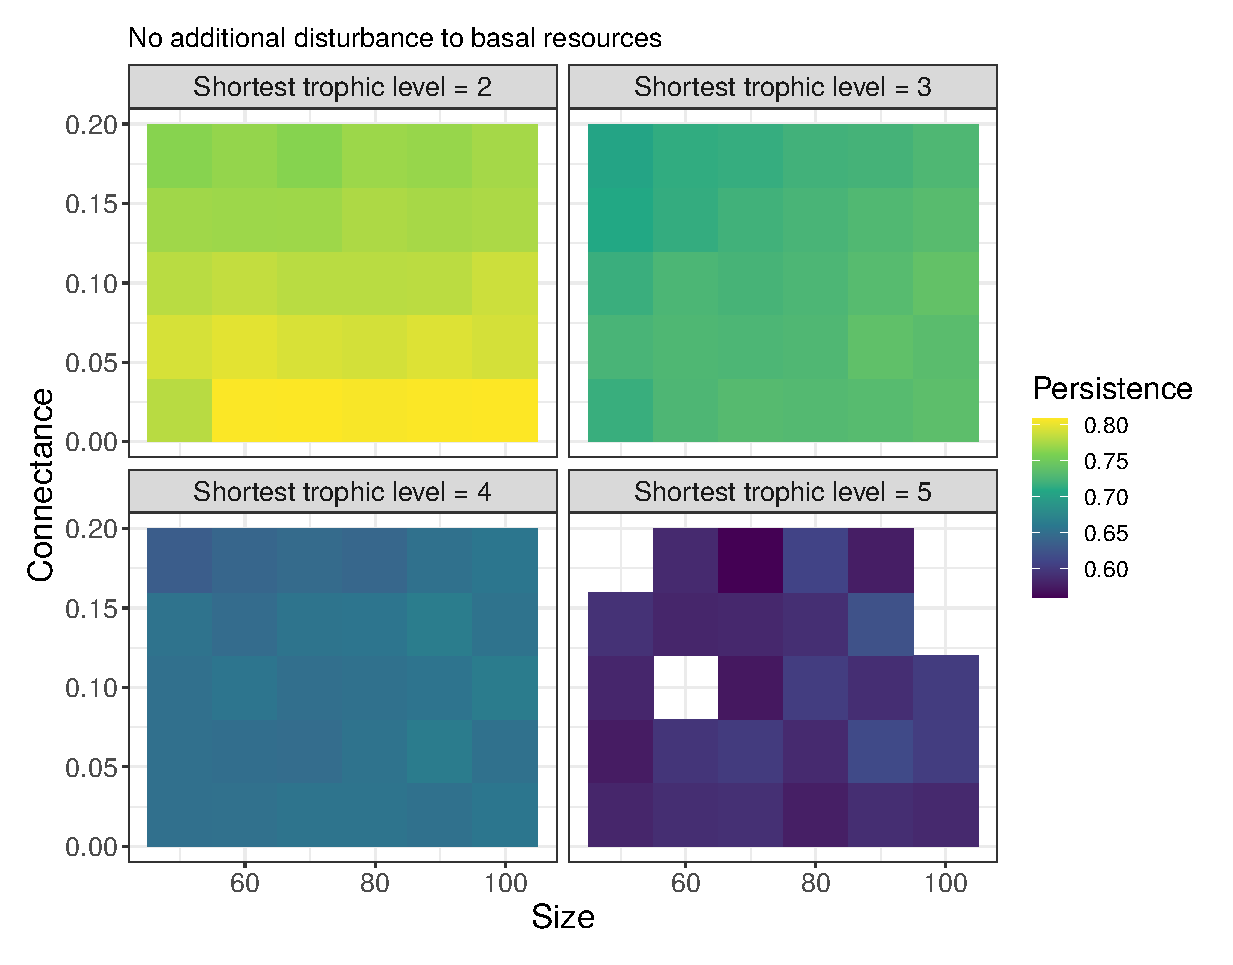
\includegraphics[width=.9\textwidth]{figures/heatmap_STL_allCS_BP0.eps}
     \caption{All species across all levels experience a risk of going extinct due to causes not related to the web of $\pi = 0.1$. The sub figures show final persistence for consumers with different shortest trophic length, for increasing connectance (y-axis) and network size (x-axis). Persistence decreases with darker color in the heat map.}
     \label{fig:heatmap_stl_BP0}
    \end{figure}


    \begin{figure}[hb!]
     \centering
     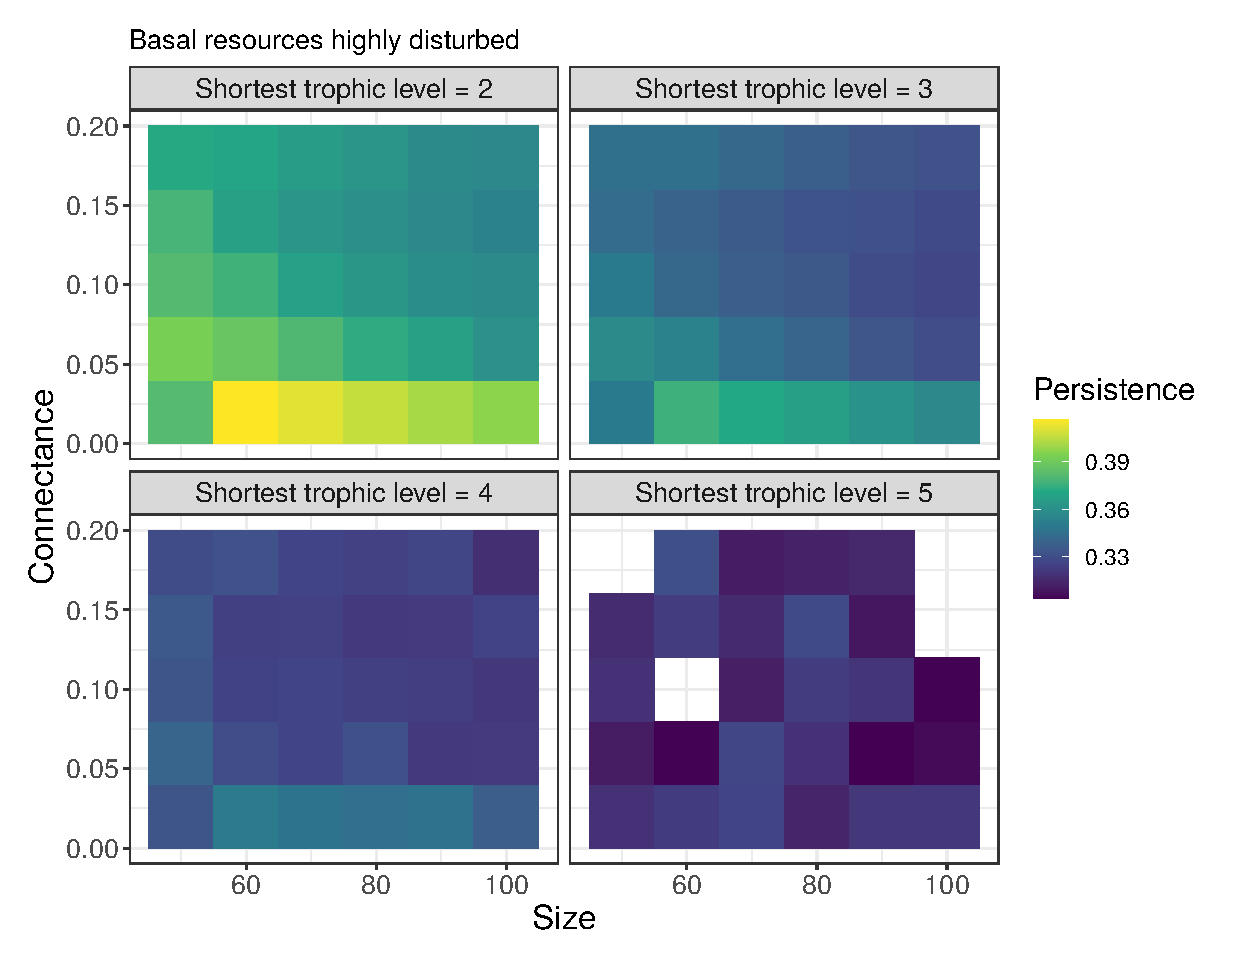
\includegraphics[width=.9\textwidth]{figures/heatmap_STL_allCS_BP1.eps}
     \caption{Basal resources experience a disturbance increasing their probability to go extinct to $\pi = 0.5$. All consumer species go extinct due to causes not related to the web itself with probability $\pi = 0.1$. The sub figures show final persistence for consumers with different shortest trophic length, for increasing connectance (y-axis) and network size (x-axis). Persistence decreases with darker color in the heat map.}
     \label{fig:heatmap_stl_BP1}
    \end{figure}

\clearpage

\section{Within-network motif-persistence relationships}

    We compared the outcomes from linear mixed-effect models (LMMs) relating persistence to motif roles across all networks (Fig. 3 and Table 1, \emph{Main Text}) with similar linear regressions (LRs) made on each single network separately.
    The main trends are similar in both analyses, but different-sized networks showed slightly different results for some motifs when considered individually (Figure~\ref{fig:density_prop_S}).
    For the three-species chain and omnivory motifs, a significant interaction between disturbance and the effect of the focal motif means that having a larger proportion of the role be made up of the chain or omnivory motif is associated with lower persistence at high levels of disturbance (Fig. 3 and Table 1, \emph{Main Text}). 
    The same pattern holds overall for LRs fit within a network  (Figure~\ref{fig:density_prop_S})
    : the fraction of negative slopes for the proportion of three-species chain and omnivory motifs increases with increasing disturbance. 
    This trend is most pronounced in large networks. (bottom panel, Figure~\ref{fig:density_prop_S}). 
    % Besides the decrease in fraction of positive slopes with increasing disturbance, the omnivory motif showed a higher overall fraction of positive slopes in comparison to the three-species chain motif, corresponding to the positive main effect of omnivory (Fig. 3 and Table 1, \emph{Main Text}). 
    
    
    \begin{figure}[hb!]
        \centering
            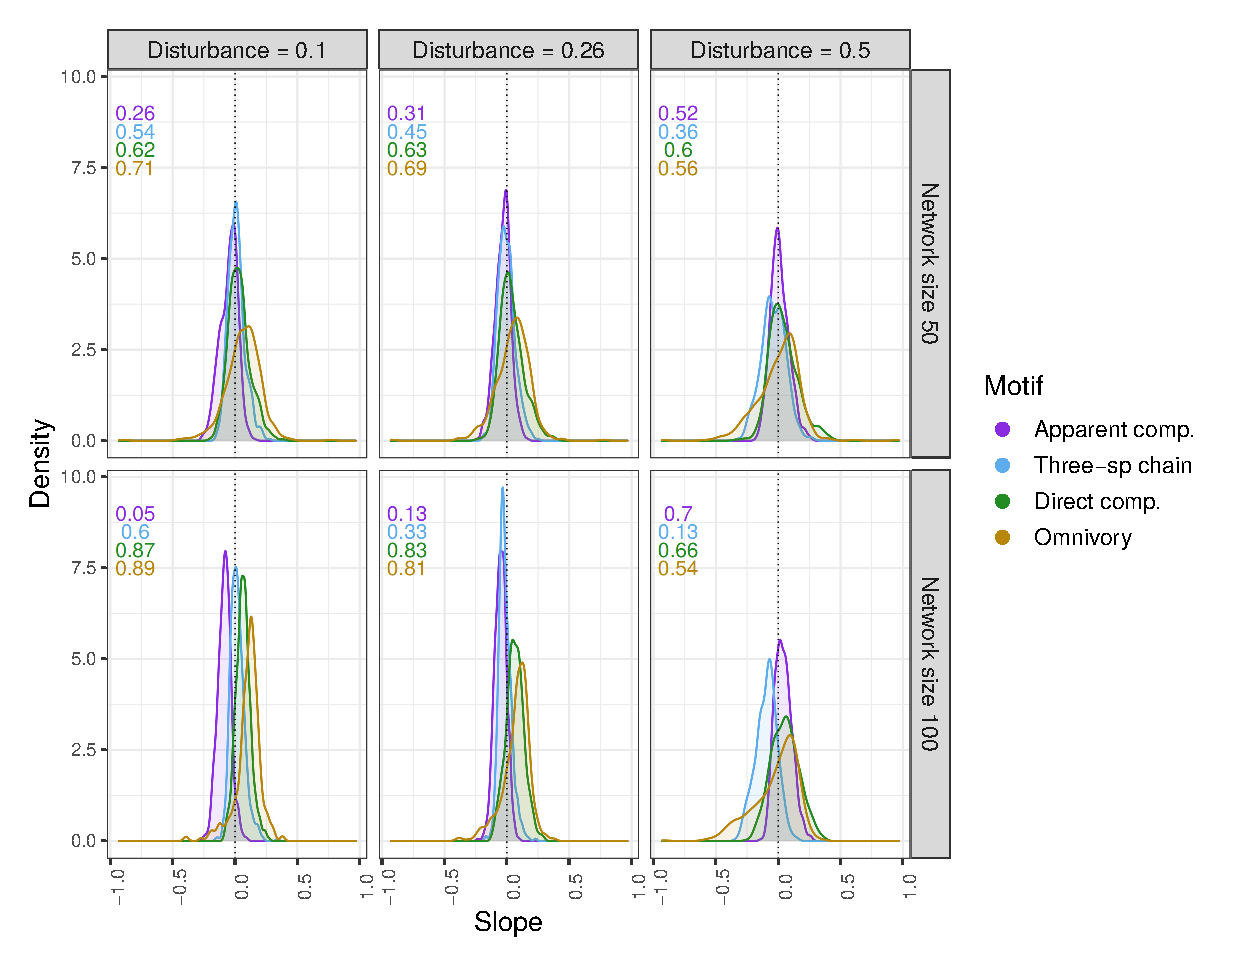
\includegraphics[width=\textwidth]{figures/prop_dens_bp_vs_S_allC.eps}
            \caption{Here we show the density (y-axis) of slopes (x-axis) of persistence against proportion of different motifs for all simulated webs of all connectances - a visualization of how an increased proportion of each motif (different colored lines) affects persistence of consumer species. Columns show the result for various disturbances on the basal level, from $\pi = 0.1$ (left) to $\pi = 0.5$ (right). Rows show various network sizes. The dotted, vertical lines indicate zero on the x-axis. A negative slope value reflects a negative relationship between increased participation in a motif and persistence, while a positive slope value reflects a positive relationship - an increased proportion of a specific motif increase persistence. The fraction of replicates with a slope greater than zero are stated in numbers in each sub-plot, the color corresponding to each motif (legend). }
            \label{fig:density_prop_S}
        \end{figure}    

    
    
    For the apparent and direct competition motifs, the LMMs include a positive interaction between disturbance and the proportion of the motif in a species' role (Fig. 3 and Table 1; \emph{Main Text}).
    This means that having more of the role made up of these two motifs is increasingly beneficial at higher levels of disturbance, a trend which is also evident from the increasing fraction of positive slopes with increasing disturbance based on LRs of each network at each level of disturbance. % (Figure~\ref{fig:density_prop_S}).
    As with the trends for omnivory and three-species chains, these increases are strongest in large networks. % (bottom row, Figure~\ref{fig:density_prop_S}).
    % For direct competition, the fraction of slopes are similar across disturbance levels. Although this interaction is not positive when accounting for network size, the fraction of positive slopes are throughout high.
    The increase in the proportion of positive slopes was much stronger for apparent competition than direct competition, consistent with the smaller (but still significant) interaction term for between direct competition in the LMMs.
    A high proportion of direct competition in a species' role tended to be associated with greater probability of persistence across levels of disturbance and network size.
    % In conclusion, species richness does not considerably alter the trends visible in the LMMs. High species richness more clearly display an interaction between motif proportion, persistences and disturbance levels, while this effect is smaller with low species richness. 
\clearpage
                
\section{Persistence and motif profiles}

    % Updated and expanded to include permanova tests
    Persistence varied with the frequencies of different motifs in a network profile ($F_{1,2998}$=645, $p$\textless0.001 for a PERMANOVA of dissimilarity in motif profiles against mean persistence).
    However, motif profiles were not evenly distributed across mean persistences ($F_{134,2865}$=1.77, $p$\textless0.001 for an ANOVA of dissimilarity in motif profiles against mean persistence, rounded to 3 decimal places).
    Specifically, motif profiles were more variable (higher dissimilarities) in networks with higher mean persistence.
    As non-homogeneous variability can cause a PERMANOVA to return a false positive~\citep{Anderson2001}, this means that we must treat our PERMANOVA result as tentative and place more weight on the single-motif regressions.


    % Updated to use mean instead of all species
    \begin{table}[hb!]
        \caption{Coefficients ($\beta$) for models relating persistence to the proportion of a network profile, the level of disturbance to basal resources (corresponding to a probability of extinction ranging between 0.1 and 0.5), and their interaction. Predictors were centered and scaled before model fitting. All effects were significant ($p$\textless0.05). We also provide the $R^2$ (multiple $R^2$). }
        \label{motif_profile_tab}
        \centering
        \begin{tabular}{c|c c c c c | c}
            Motif & Intercept & Proportion & Disturbance & Interaction & $R^2$\\
            \hline
            Omnivory & 0.574 & -0.0140 & -0.139 & -5.59$\times10^{-4}$ & 0.968 \\
            Apparent competition & 0.574 & 0.0112 & -0.139 & 5.90$\times10^{-4}$ & 0.964 \\
            Direct competition & 0.574 & 3.38$\times10^{-3}$ & -0.139 & 1.81$\times10^{-4}$ & 0.958 \\
            Three-species chain & 0.574 & 5.80$\times10^{-3}$ & -0.138 & -3.07$\times10^{-5}$ & 0.960 \\ 
        \end{tabular}
    \end{table}
\clearpage


\section{Motif profiles and global properties}
    % No update needed

    A network's normalized motif profile (i.e., proportions of the total made up by each motif) was related to the network's size, connectance, and the interaction between them ($F_{1,2996}$=74.3, $p$\textless0.001; $F_{1,2996}$=4203, $p$\textless0.001; and $F_{1,2996}$=27.8, $p$\textless0.001, respectively in a PERMANOVA of dissimilarity in normalized network motif profiles against network size, connectance, and their interaction).
    However, normalized motif profiles were not homogeneously variable across levels of network size, connectance, or their interaction  ($F_{5,2994}$=16.8, $p$\textless0.001; $F_{4,2995}$=31.7, $p$\textless0.001; and $F_{29,2970}$=11.9, $p$\textless0.001 for ANOVAs of dispersion of motif profiles against size, connectance, and combinations of size and connectance, respectively).These differences in variability can cause false positives in the PERMANOVA test. Variability was highest in small and low-connectance networks (Fig.~\ref{dispersion_normmotifs}).


   \begin{figure}[hb!]
       \centering
       \includegraphics[width=.75\textwidth]{figures/proportion_profile_dispersion.eps}
       \caption{Dispersion of normalized motif profiles (i.e., proportions of each motif) within a network about the centroid for that combination of network size and connectance. Each circle represents a single network; circle colour indicates network size. Scatter has been introduced about each level of connectance to increase visual clarity; the levels of connectance we consider are indicated by vertical black lines.}
       \label{dispersion_normmotifs}
    \end{figure}


    The frequencies of the four possible motifs were related to global network properties.

    \begin{table}[hb!]
        \centering
        \caption{Coefficients for linear regressions relating the proportion of each motif in the total motif profile of a network to network size, connectance, and their interaction. Coefficients in \textbf{bold} are significant (\textless0.05).}
       \label{network_prop_lms}
       \begin{tabular}{c|c c c c c}
            Motif & Intercept & Size & Connectance & Interaction \\
            \hline
            Three-species Chain & \textbf{0.262} & \textbf{1.78$\times10^{-4}$} & \textbf{-0.157} & \textbf{-3.27$\times10^{-3}$} \\
            Apparent Competition & \textbf{0.541} & \textbf{-5.06$\times10^{-4}$} & \textbf{-1.00} & \textbf{2.59$\times10^{-3}$} \\
            Direct Competition & \textbf{0.193} & -3.56$\times10^{-5}$ & \textbf{-0.556} & \textbf{5.92$\times10^{-3}$} \\
            Omnivory & 4.82$\times10^{-3}$ & \textbf{3.64$\times10^{-4}$} & \textbf{1.71} & \textbf{-5.24$\times10^{-3}$}\\
            \hline
            \end{tabular}
    \end{table}        
\clearpage
    
            

\section{Persistence and global network properties}

    Connectance and species richness had smaller effects on consumer persistence than disturbance (Figs.~\ref{fig:lm_CS}, \ref{fig:heatmap_CS}, Table~\ref{tab:per_vs_SC}).

    % updated to use network means rather than all species
    \begin{figure}[hb!]
        \centering
        \includegraphics[width=\textwidth]{figures/persistence_vs_SC_lm.eps}
        \caption{Persistence decreased strongly with increasing probability of disturbance to basal resources, while network size, connectance, and their interaction had smaller effects. \textbf{A)} Persistence decreased slightly with increasing network size at high levels of disturbance, increased slightly with increasing network size at low levels of disturbance, and did not vary noticeably with network size at moderate levels of disturbance. Networks with lower connectance (dotted line) had slightly higher persistence than networks with moderate (solid line) or high (dashed line) connectance.
        \textbf{B)} Persistence decreased with increasing connectance for all levels of disturbance and network size. Network size (line types) did not strongly affect these relationships.}
        \label{fig:lm_CS}
    \end{figure}



    \begin{figure}[hb!]
      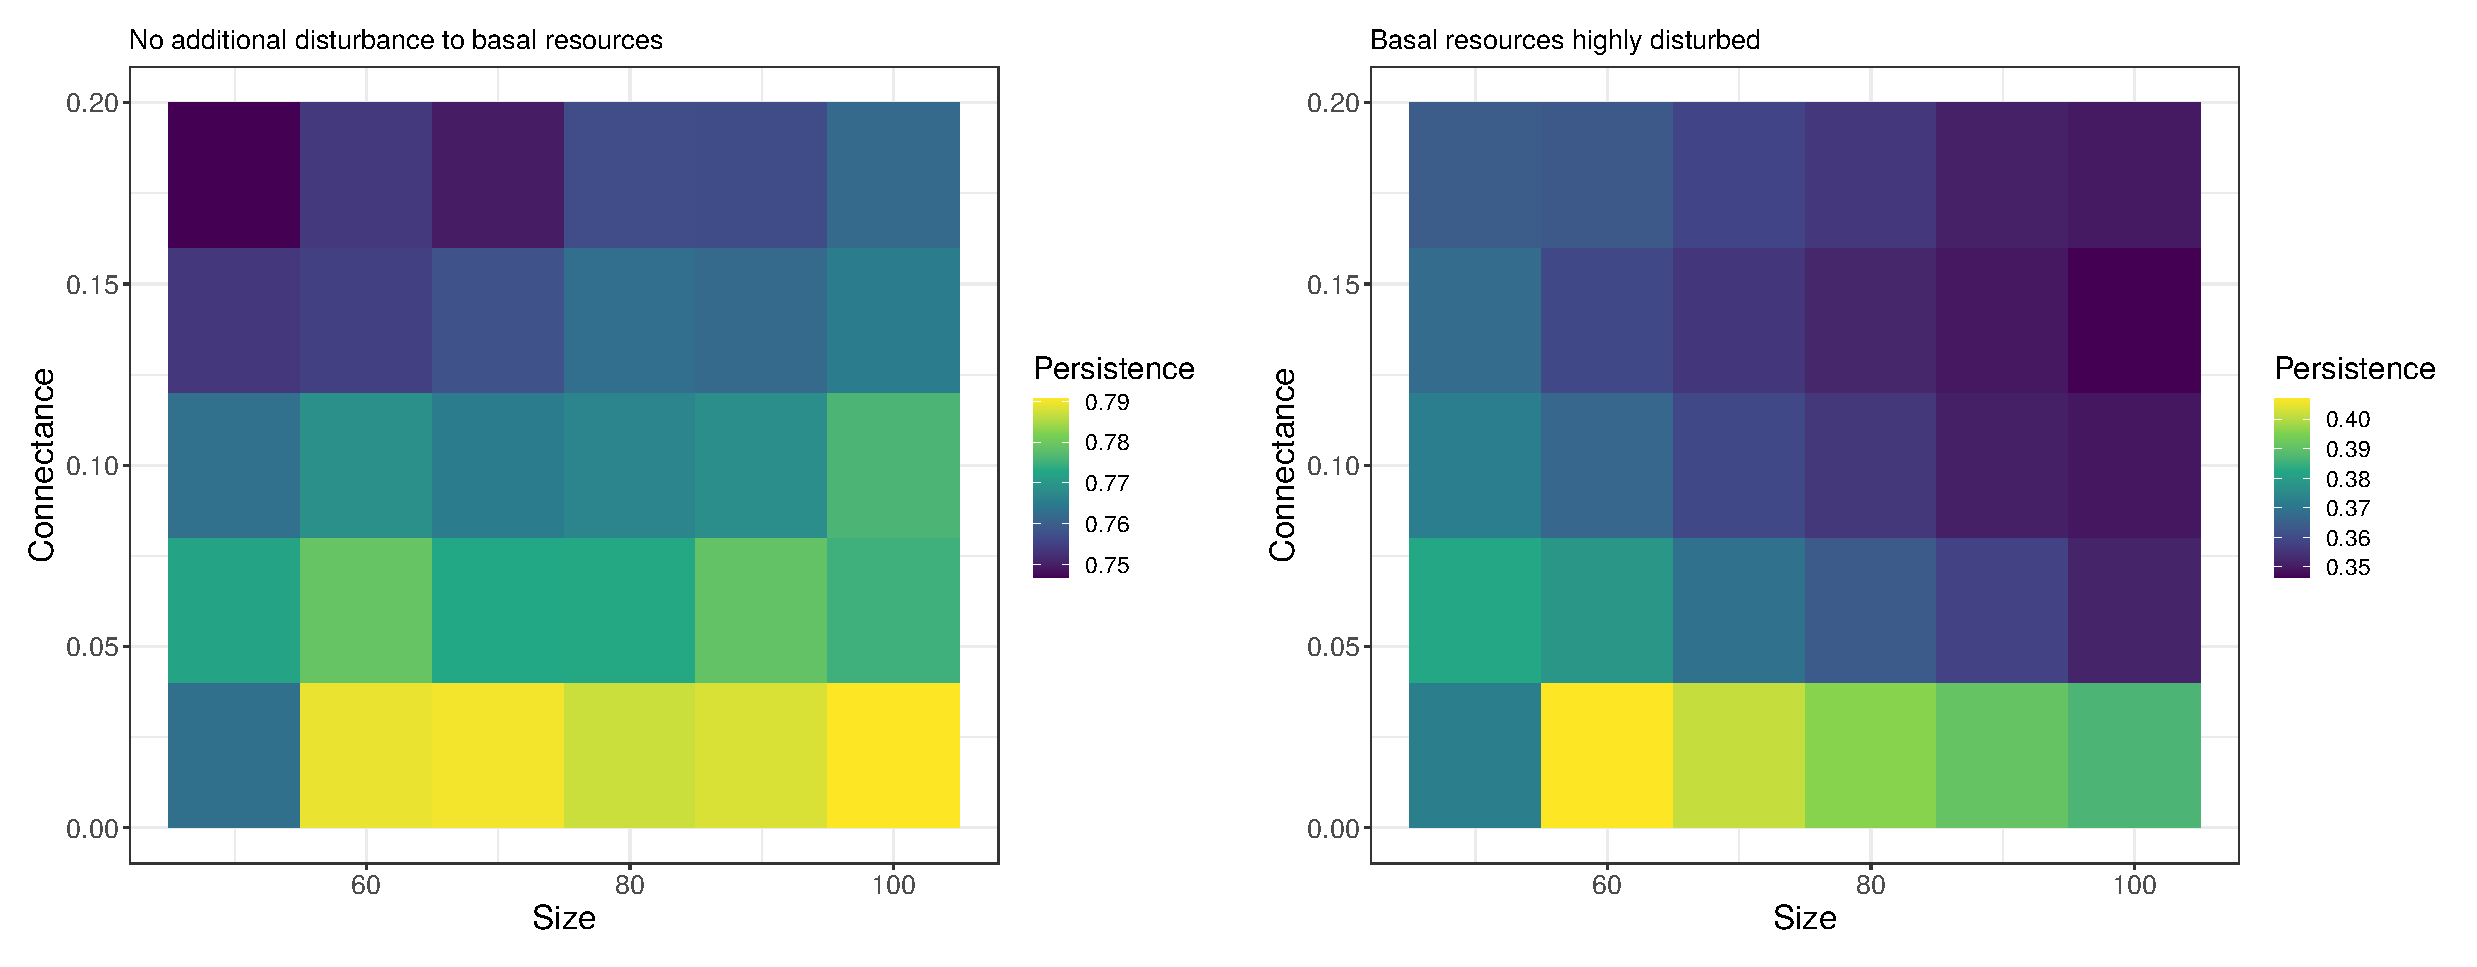
\includegraphics[width=\textwidth]{figures/heatmap_CS_BPcompare.eps}
       \caption{Heat maps of average consumer persistence in networks with varying connectance (y-axis) and network size (x-axis) at two levels of disturbance to basal resources. Persistence decreases with darker color in the heat map. When basal species are not disturbed, all species experience a baseline extinction risk of $\pi = 0.1$. When basal species are highly disturbed, their baseline extinction risk rises to $\pi = 0.5$ while the baseline risk of consumers is not changed.}
       \label{fig:heatmap_CS}
    \end{figure}


    % Updated to use mean rather than all species.
    \begin{table}[hb!]
        \caption{Mean persistence of consumers within a network depends on network size (S) and connectance (C), the level of disturbance to basal resources (D), and interactions between them. Here we show the effect sizes ($\beta$) and $p$-values for the regression described above. All predictors were centered and scaled before fitting the model. The level of disturbance corresponds to basal resources having a probability of extinction ranging between $0.1 - 0.5$ (see \emph{Methods}).
        }
        \label{tab:per_vs_SC}
        \centering
        \begin{tabular}{c|c c |}
            Predictor & $\beta$ & $p$-value \\
            \hline
            Intercept & 0.574 & \textless0.001 \\
            Size & -4.82$\times10^{-4}$  & 0.011 \\
            Connectance & -0.0137 & \textless0.001 \\
            Disturbance & -0.139 & \textless0.001 \\
            S:C & -9.77$\times10^{-4}$ & \textless0.001 \\
            S:D & -3.46$\times10^{-3}$ & \textless0.001 \\
            C:D & -2.25$\times10^{-4}$ & 0.233 \\
            S:C:D: & -3.97$\times10^{-4}$ & 0.036 \\
        \end{tabular}
    \end{table}

\clearpage

\section{Glossary}

 \begin{table}[hb!]
 \label{glossary}
 \caption{Glossary of terms relating to motifs and Bayesian networks}
     \footnotesize{
 \begin{tabular}{l|m{11cm}}
     Term & Definition \\
     \hline
     Global property & A property of the whole network (e.g., species richness) \\
     Local property & A property of a single species, generally referring only to direct interactions (e.g., degree) \\
     Meso-scale property &  A property of a single species which includes direct and indirect interactions; the species' immediate `neighbourhood' in the network (e.g., motif participation) \\
     Motif & Set of $n$ interacting species. In this case, $n=3$ \\
     Network motif profile & Vector describing the frequency of each motif in the network. \\
     & Normalised by dividing counts of each motif by the total across all motifs.\\
     Motif participation role & Vector describing the frequency with which a focal species appears in each motif.\\
     & Normalised by dividing counts for each motif by the total across all motifs. \\
     Bayesian network & A directed acyclic graph, used to predict species' likelihood of persistence. \\
     Network mean persistence & The mean likelihood of persistence for all consumers in a network.\\
     Species persistence & The individual likelihood of a species not going extinct.\\
     In-degree & Number of prey species to a consumer species.\\
     Trophic level (STL) & The shortest food chain between the focal species and any basal species.\\
     Disturbance ($\pi_{disturbed}$) & Probability of extinction of a basal resource when extra disturbance is added. \\
     Baseline extinction &  When no disturbance is applied, $\pi_{base}$=0.1.\\
 \end{tabular}}
 \end{table}
 
\clearpage 

% \section{SH: Persistence and motif roles}

%     \subsection*{Methods}

%         As one more level of detail, we can consider the frequency with which a species appears in each \emph{position} in each motif. 
%         Different positions are associated with different numbers of predators and prey, making the similarities and differences between motifs and degree more explicit.
%         The full set of these positions, across all motifs, is the species' \emph{motif role}~\citep{Stouffer2010,Cirtwill2017}.
%         As with motif participation, we normalized motif roles by dividing the number of times a species appeared in each position by the total number of times it appeared in all positions~\citep{Baker2015,Cirtwill2017}.
        
        
%         [[Could add a PERMANOVA to show that species' roles overal affect their persistence. Haven't done so yet.]]
        

%         To test whether participating in different motif positions was related to a species' probability of persistence, we fit similar models to those for motif participation.
%         For each position, we fit a linear mixed-effect model relating persistence to the frequency of the position in a species' motif role, disturbance, and their interaction.
%         To account for differences in persistence across networks of different size and connectance, we included a random effect of the interaction between size and connectance.
%         All regressions were fit using the R~\citep{R} function `lmer' from the package \emph{lmerTest}~\citep{lmerTest}.

    
%     \subsection*{Results}

%     \begin{table}[h!]
%         \caption{Coefficients in a series of regressions relating probability of persistence to the frequency of a position in a species' motif role, disturbance, and their interaction. For ease of comparison between motifs, we did not center or scale predictors. Note, however, that some motifs and positions have higher frequencies than others.}
%         \label{tab:persistence_vs_positions}
%         \centering
%         \begin{tabular}{l | c c c c}
%         Position    & Intercept & Disturbance   & Position  & Interaction \\
%         \hline
%         Chain: top  & 0.880 &   -0.985 & -0.00544 & -0.332 \\
%         Chain: bottom   & 0.883 &   -1.07 & -0.0510 &   0.647 \\
%         Chain: middle   & 0.862 & -1.00 &   0.246 & -0.244 \\
%         \hline
%         Dir. Comp.: top & 0.872 &   -0.995  & 0.0549 &  -0.178 \\
%         Dir. Comp.: bottom & 0.886 &    -1.07 & -0.113 &    0.939 \\
%         \hline
%         Omnivory: top   & 0.872 &   -0.984 &    0.180 & -0.818 \\
%         Omnivory: middle & 0.873 & -1.00 &  0.119 & -0.324 \\
%         Omnivory: bottom & 0.882 & -1.06 &  -0.0449 &   0.845 \\
%         \hline
%         App. Comp.: top & 0.865 &   -0.966 &    0.140 & -0.520 \\
%         App. Comp.: bottom & 0.910 &    -1.12 & -0.100 &    0.323 \\
%         \hline
%         \end{tabular}
%     \end{table}


%     \begin{figure}
%         \centering
%         \includegraphics[width=0.75\textwidth]{figures/persistence_positions_Apparent.eps}
%         \caption{A species' probability of persistence varied with the frequency of different motif positions in its role. Here we show the relationships between persistence and the proportions of the three positions in the apparent competition motif at three levels of probability of extinction for basal resources (p=0.1, 0.26, and 0.42), indicated by line colour. Line style indicates the motif  position. }
%         \label{fig:apparent_positions}
%     \end{figure}

%     \begin{figure}
%         \centering
%         \includegraphics[width=0.75\textwidth]{figures/persistence_positions_Direct.eps}
%         \caption{A species' probability of persistence varied with the frequency of different motif positions in its role. Here we show the relationships between persistence and the proportions of the three positions in the direct competition motif at three levels of probability of extinction for basal resources (p=0.1, 0.26, and 0.42), indicated by line colour. Line style indicates the motif  position. }
%         \label{fig:direct_positions}
%     \end{figure}
    
    
%     \begin{figure}
%         \centering
%         \includegraphics[width=0.75\textwidth]{figures/persistence_positions_Three-species.eps}
%         \caption{A species' probability of persistence varied with the frequency of different motif positions in its role. Here we show the relationships between persistence and the proportions of the three positions in the three-species chain motif at three levels of probability of extinction for basal resources (p=0.1, 0.26, and 0.42), indicated by line colour. Line style indicates the motif  position. }
%         \label{fig:chain_positions}
%     \end{figure}
        
% \clearpage

% \section{SI: Motif roles and network properties}

%     \subsection*{Methods}
    
%         As with network motif profiles and motif participation, species' motif roles may vary with network size and connectance and with the species' in degree and trophic level.
%         To identify these relationships, we fit two linear regressions for each motif position.
%         The first related the frequency of the position in species' roles to network size, connectance, and their interaction.
%         The second related the frequency of the position to in-degree, STL, and their interaction.
%         All regressions were fit using the R~\citep{R} base function `lm'.
        
        
%     \subsection*{Results}
%         \subsection*{Degree and trophic level}
    
%             Positions in all three motifs were strongly related to in-degree and/or trophic level (Table~\ref{DT_tab}).
%             The top position in the omnivory motif increased with increasing degree across all trophic levels.
%             The frequency of the middle position increased with the interaction of degree and trophic level.
%             The bottom position was generaly rare, especially for species with high degree or high trophic level (this suggests that the bottom position is frequently a basal resource).
            
            
%             The frequency of the bottom position in the apparent competition motif decreased strongly with increasing degree, especially for species at a high trophic level.
%             The frequency of the top position increased strongly with increasing degree and was not strongly related to trophic level.
            
            
%             The frequency of the bottom position in the direct competition motif increased with increasing degree, especially for species at a high trophic level.
%             The bottom position was very rare, especially for species with high degree (also suggesting that this position is usually a basal resource).
            
            
%             The bottom position in the three-species chain was generally rare, especially for species with high degree or trophic level (again, this is likely to commonly be basal resources).
%             The middle position in the three-species chain did not vary strongly with degree and declined slightly with increasing trophic level.
%             The top position in the three-species chain increased with trophic level, degree, and their interaction.
    
%             \begin{table}[h!]
%                 \caption{Coefficients ($\beta$) and $p$-values for linear regressions of the frequency of each motif position against in-degree, STL, and their interaction.}
%                 \label{DT_tab}
%                 \footnotesize
%                 \begin{tabular}{c c | c c | cc | cc |}
%                 Motif & Position & \multicolumn{2}{c}{Degree} & \multicolumn{2}{c}{STL} & \multicolumn{2}{c}{Interaction} \\
%                 & & $\beta$ & $p$ & $\beta$ & $p$ & $\beta$ & $p$ \\
%                 \hline
%                 Chain & bottom & -1.47 $\times10^{-5}$ & 0.769 & -0.0218 & \textless0.001 & -0.00160 & \textless0.001 \\
%                 Chain & middle & 3.13$\times10^{-4}$ & \textless0.001 & -0.0353 & \textless0.001 & 1.85$\times10^{-5}$ & 0.275 \\
%                 Chain & top & -0.0172 & \textless0.001 & 0.0259 & \textless0.001 & 0.00919 & \textless0.001 \\
%                 \hline
%                 Omnivory & bottom & 6.14$\times10^{-4}$ & \textless0.001 & -0.00270 & \textless0.001 & -0.00112 & \textless0.001 \\
%                 Omnivory & middle & 3.13$\times10^{-4}$ & \textless0.001 & -0.0353 & \textless0.001 & 1.85$\times10^{-5}$ & \textless0.001 \\
%                 Omnivory & top & 0.00413 & \textless0.001 & 0.00381 & \textless0.001 & 9.96$\times10^{-5}$ & \textless0.001 \\
%                 \hline
%                 App. comp. & bottom & -4.74$\times10^{-4}$ & \textless0.001 & -0.663 & \textless0.001 & 0.00224 & \textless0.001 \\
%                 App. comp. & top & 2.12$\times10^{-5}$ & 0.183 & -0.112 & \textless0.001 & -4.47$\times10^{-4}$ & \textless0.001 \\
%                 \hline
%                 Dir. comp. & bottom & 8.12$\times10^{-4}$ & \textless0.001 & -5.57$\times10^{-3}$ & \textless0.001 & -1.37$\times10^{-3}$ & \textless0.001 \\
%                 Dir. comp. & top & -0.00405 & \textless0.001 & -0.0435 & \textless0.001 & 0.00260 & \textless0.001 \\
%                 \hline
%                 \end{tabular}
%                 \end{table}
    
    
%             \begin{figure}[h!]
%                 \centering
%                 \includegraphics[width=.75\textwidth]{figures/positions_byTL_Omnivory.eps}
%                 \caption{The frequencies of positions within the omnivory motif varied with degree, trophic level, and their interaction.}
%                 \label{omnivory_DT}
%             \end{figure}
    
    
%             \begin{figure}[h!]
%                 \centering
%                 \includegraphics[width=.75\textwidth]{figures/positions_byTL_Apparentcompetition.eps}
%                 \caption{The frequencies of positions within the apparent competition motif varied with degree, trophic level, and their interaction.}
%                 \label{appcomp_DT}
%             \end{figure}
    
%             \begin{figure}[h!]
%                 \centering
%                 \includegraphics[width=.75\textwidth]{figures/positions_byTL_Directcompetition.eps}
%                 \caption{The frequencies of positions within the direct competition motif varied with degree, trophic level, and their interaction.}
%                 \label{dircomp_DT}
%             \end{figure}
    
    
%             \begin{figure}[h!]
%                 \centering
%                 \includegraphics[width=.75\textwidth]{figures/positions_byTL_Three-specieschain.eps}
%                 \caption{The frequencies of positions within the three-species chain motif varied with degree, trophic level, and their interaction.}
%                 \label{chain_DT}
%             \end{figure}
    
    
%         \subsection*{Network size and connectance}
    
%             % Many of these are significant, but the slopes tend to be very shallow. TL and degree are more interesting - this is DEFINITELY SI.
%             The frequency of the top position in the apparent competition motif did not vary strongly with network size or connectance (Table~\ref{SC_tab}).
%             The frequency of the bottom position in the apparent competition motif decreased with increasing connectance but did not vary strongly vary with network size.
            
            
%             The frequency of the top position in the direct competition motif increased slightly with the interaction of network size and connectance (i.e., in large and highly-connected networks).
%             The frequency of the bottom position in the direct competition motif was low in all networks.
            
            
%             The frequency of all three positions in the omnivory motif showed similar relationships with network size and connectance.
%             Frequencies of these motifs increased with increasing connectance and were not strongly affected by network size.
%             None of the positions in the three-species chain varied strongly with network size or connectance.
    
    
%             \begin{table}[h!]
%                 \caption{Coefficients ($\beta$) and $p$-values for linear regressions of the frequency of each motif position against network size, connectance, and their interaction.}
%                 \label{SC_tab}
%                 \footnotesize
%                 \begin{tabular}{c c | c c | cc | cc |}
%                 Motif & Position & \multicolumn{2}{c}{Size} & \multicolumn{2}{c}{Connectance} & \multicolumn{2}{c}{Interaction} \\
%                 & & $\beta$ & $p$ & $\beta$ & $p$ & $\beta$ & $p$ \\
%                 \hline
%                 Chain & bottom & -4.63$\times10^{-5}$ & \textless0.001 & -0.108 & \textless0.001 & -1.94$\times10^{-4}$ & 0.035 \\
%                 Chain & middle & 1.68$\times10^{-4}$ & \textless0.001 & -0.0530 & \textless0.001 & -0.00212 & \textless0.001 \\
%                 Chain & top & 1.00$\times10^{-4}$ & \textless0.001 & 0.0304 & 0.015 & -8.79$\times10^{-4}$ & \textless0.001 \\
%                 \hline
%                 Omnivory & bottom & 2.00$\times10^{-4}$ & \textless0.001 & 0.575 & \textless0.001 & -0.00240 & \textless0.001 \\
%                 Omnivory & middle & 1.32$\times10^{-4}$ & \textless0.001 & 0.551 & \textless0.001 & -0.00215 & \textless0.001 \\
%                 Omnivory & top & 6.42$\times10^{-5}$ & \textless0.001 & 0.448 & \textless0.001 & -0.00115 & \textless0.001 \\
%                 \hline
%                 App. comp. & bottom & -4.74$\times10^{-4}$ & \textless0.001 & -0.663 & \textless0.001 & 0.00224 & \textless0.001 \\
%                 App. comp. & top & 2.12$\times10^{-5}$ & 0.183 & -0.112 & \textless0.001 & -4.47$\times10^{-4}$ & \textless0.001 \\
%                 \hline
%                 Dir. comp. & bottom & 7.94$\times10^{-5}$ & \textless0.001 & -0.0663 & \textless0.001 & 0.00101 & \textless0.001 \\
%                 Dir. comp. & top & -2.45$\times10^{-4}$ & \textless0.001 & -0.602 & \textless0.001 & 0.00610 & \textless0.001 \\
%                 \hline
%                 \end{tabular}
%                 \end{table}
    
    
%             \begin{figure}[h!]
%                 \centering
%                 \includegraphics[width=.75\textwidth]{figures/positions_bySC_Omnivory.eps}
%                 \caption{The frequencies of positions within the omnivory motif varied with degree, trophic level, and their interaction.}
%                 \label{omnivory_SC}
%             \end{figure}
    
    
%             \begin{figure}[h!]
%                 \centering
%                 \includegraphics[width=.75\textwidth]{figures/positions_bySC_Apparentcompetition.eps}
%                 \caption{The frequencies of positions within the apparent competition motif varied with degree, trophic level, and their interaction.}
%                 \label{appcomp_SC}
%             \end{figure}
    
%             \begin{figure}[h!]
%                 \centering
%                 \includegraphics[width=.75\textwidth]{figures/positions_bySC_Directcompetition.eps}
%                 \caption{The frequencies of positions within the direct competition motif varied with degree, trophic level, and their interaction.}
%                 \label{dircomp_SC}
%             \end{figure}
    
    
%             \begin{figure}[h!]
%                 \centering
%                 \includegraphics[width=.75\textwidth]{figures/positions_bySC_Three-specieschain.eps}
%                 \caption{The frequencies of positions within the three-species chain motif varied with degree, trophic level, and their interaction.}
%                 \label{chain_SC}
%             \end{figure}
    
    
%     \clearpage
    
% \clearpage 

% \section*{SJ: Proportion of basal resources in the network}

%     \subsection*{Basal resources and mean persistence}

%         We fit a linear regression relating consumer persistence to network size, connectance, disturbance, the proportion of the network made up of basal resources (pBasal), and all interactions between them. All terms were significant, indicating that the pBasal affects a consumer's probability of persistence but that this effect depends upon other aspects of network structure.
%         As with the effects of network size and connectance, however, the effects of pBasal were small in the range of networks we considered here (Fig.~\ref{fig:lm_BCS}).
%         % Table is from basal_models.Rdata: BCper, if we want it.
    
%         \begin{figure}[h!]
%             \centering
%             \includegraphics[height=0.75\textheight]{figures/persistence_vs_BSC_lm.eps}
%             \caption{Persistence decreased strongly with increasing probability of disturbance to basal resources, while the proportion of the network made up of basal resources, network size, connectance, and their interactions had smaller effects. We show relationships with persistence for low disturbance ($\pi$=0.1) and high disturbance($\pi$=0.5). For each predictor other than disturbance, we show the relationship between the focal predictor and persistence for combinations of the lowest and highest observed values of the other predictors. For proportion of basal resources, these values were 0.02 and 0.5; for network size, 50 and 100; and for connectance, 0.02 and 0.18.}
%             \label{fig:lm_BCS}
%         \end{figure}
    

%     \subsection*{Motif profiles and proportion of basal resources}
    
%         We repeated our analyses testing whether motif profiles were related to network size and connectance, replacing network size with the proportion of the network made up by basal resources (pBasal).
%         A network's overall motif profile was significantly related to pBasal ($F_{1,2996}$=196, $p$\textless0.001, connecance ($F_{1,2996}$=10.0, $p$\textless0.001), and their interaction ($F_{1,2996}$=27.3, $p$\textless0.001).
%         However, this result could be a false positive as the dispersion of motif profiles was non-homogeneous across connectance ($F_{4,2995}$=5.17, $p$\textless0.001), pBasal ($F_{128,2871}$=19.0, $p$\textless0.001), and their interaction ($F_{291,2708}$=13.4, $p$\textless0.001).
%         Distance from group centroids was low for networks with extremely low or extremely high pBasal, perhaps because there were few such networks.
%         The ranges and median distances from group centroids was similar across levels of connectance.
        
        
%         Considered separately, the proportions of all four motifs in a network's motif profile were related to the proportion of basal resources in a network (Fig.~\ref{fig:Blms}).
%         The proportion of the three-species chain decreased in networks with more basal resources ($\beta_{pBasal}$=-0.080, $p$\textless0.001) and networks with higher connectance ($\beta_{C}$=0.498, $p$\textless0.001).
%         The interaction between pBasal and connectance was not significant ($\beta_{pBasal:C}$=0.0554, $p$=0.766).
        

%         The proportion of the omnivory motif decreased in networks with more basal resources ($\beta_{pBasal}$=-0.198, $p$\textless0.001), increased in networks with higher connectance ($\beta_{C}$=0.895, $p$\textless0.001), and increased most strongly in networks with high connectance and many basal resources ($\beta_{pBasal:C}$=2.53, $p$\textless0.001).   
        
%         The proportion of the apparent competition motif increased with in networks with more basal resources ($\beta_{pBasal}$=0.202, $p$\textless0.001) and decreased in more connected networks ($\beta_C$=-0.596, $p$\textless0.001). 
%         The interaction between the proportion of basal resources and connectance was not significant ($\beta_{pBasal:C}$=0.258, $p$\textless0.001).
        
        
%         The proportion of the direct competition motif increased in networks with more basal resources ($\beta_{pBasal}$=0.0759, $p$\textless0.001) and more-connected networks ($\beta_C$=0.199, $p$\textless0.001), but decreased with the interaction between them ($\beta_{pBasal:C}$=-2.85, $p$\textless0.001).

        
%         \begin{figure}
%             \centering
%             \includegraphics[width=.75\textwidth]{figures/motif_proportion_basal_lms.eps}
%             \caption{Mean proportion of each motif in a network's motif profile varied with connectance and the proportion of basal resources in the network. For direct competition and omnivory, the frequency of the motif also varied with the interaction between connectance and basal resources.}
%             \label{fig:Blms}
%         \end{figure}    


%     \subsection*{Motif participation and proportion of basal resources}
    
%         We fit regressions relating the proportion of each motif in a consumer's motif participation vector to the proportion of basal resources in the network (pBasal), connectance, and the interaction between them.
%         Participation in all four motifs was significantly related to pBasal, connectance, and the interaction between them (Fig.~\ref{fig:basal_participation}).
%         These interactions were strongest for apparent and direct competition.
        
%         \begin{figure}
%             \centering
%             \includegraphics[height=.65\textheight]{figures/participation_vs_BC.eps}
%             \caption{The proportion of each motif in a consumer's participation vector varied with the proportion of the network made up by basal resources, connectance, and their interaction.}
%             \label{fig:basal_participation}
%         \end{figure}
        
%         Participation in the three-species chain increased in networks with more basal resources ($\beta_{pBasal}$=0.0447, $p$\textless0.001), decreased in more-connected networks ($\beta_C$=-0.296, $p$\textless0.001), and decreased with the interaction between them ($\beta_{pBasal:C}$=-0.525, $p$\textless0.001).
%         Participation in the omnivory motif decreased in networks with more basal resources ($\beta_{pBasal}$=-0.198, $p$\textless0.001), increased in more-connected networks ($\beta_C$=0.701, $p$\textless0.001), and increased strongly with the interaction between them ($\beta_{pBasal:C}$=2.81, $p$\textless0.001).
%         Participation in the apparent competition motif decreased in networks with more basal resources and more-connected networks ($\beta_{pBasal}$=-0.0825, $p$\textless0.001 and $\beta_C$=-0.846, $p$\textless0.001) but increased strongly with the interaction between them ($\beta_{pBasal:C}$=1.66, $p$\textless0.001).
%         Participation in the direct competition motif increased in networks with more basal resources and more-connected networks ($\beta_{pBasal}$=0.235, $p$\textless0.001 and $\beta_C$=0.442, $p$\textless0.002), but decreased strongly with the interaction between them ($\beta_{pBasal:C}$=-3.94, $p$\textless0.001).
        
    
%     \subsection*{Frequencies of positions and proportion of basal resources}

%         As with the frequencies of each motif in a species' motif participation vector, the frequencies of positions in a species' motif role varied with the proportion of basal resources in the network, connectance, and their interaction (Table~\ref{BC_tab}).
        

%         \begin{table}[h!]
%             \caption{Coefficients ($\beta$) and $p$-values for linear regressions of the frequency of each motif position against the proportion of the network made up of basal resources (pBasal), connectance, and their interaction.}
%             \label{BC_tab}
%             \footnotesize
%             \begin{tabular}{c c | c c | cc | cc |}
%             Motif & Position & \multicolumn{2}{c}{pBasal} & \multicolumn{2}{c}{Connectance} & \multicolumn{2}{c}{Interaction} \\
%             & & $\beta$ & $p$ & $\beta$ & $p$ & $\beta$ & $p$ \\
%             \hline
%             Chain & bottom & -0.116 & \textless0.001 & -0.266 & \textless0.001 & 0.217 & \textless0.001 \\
%             Chain & middle & 0.0779 & \textless0.001 & -0.107 & \textless0.001 & -0.386 & \textless0.001 \\
%             Chain & top & 0.0829 & \textless0.001 & 0.0776 & \textless0.001 & -0.356 & \textless0.001 \\
%             \hline
%             Omnivory & bottom & -0.104 & \textless0.001 & 0.203 & \textless0.001 & 0.937 & \textless0.001 \\
%             Omnivory & middle & -0.0668 & \textless0.001 & 0.217 & \textless0.001 & 1.24 & \textless0.001 \\
%             Omnivory & top & -0.0269 & \textless0.001 & 0.281 & \textless0.001 & 0.638 & \textless0.001 \\
%             \hline
%             App. comp. & bottom & -0.237 & \textless0.001 & -0.874 & \textless0.001 & 1.76 & \textless0.001 \\
%             App. comp. & top & 0.154 & \textless0.001 & 0.0279 & \textless0.001 & -0.0947 & 0.013 \\
%             \hline
%             Dir. comp. & bottom & -0.0631 & \textless0.001 & -0.0247 & \textless0.001 & -0.418 & \textless0.001 \\
%             Dir. comp. & top & 0.298 & \textless0.001 & 0.466 & \textless0.001 & =3.53 & \textless0.001 \\
%             \hline
%             \end{tabular}
%             \end{table}
% \clearpage        

% \section*{SK: Motif profiles in different network sets}

%     Not all motifs were equally likely to occur in the networks we considered. 
%     Across the initially stable, acyclic networks (i.e., those used in the main text), the omnivory motif tended to make up a smaller proportion of the motif profile than other motifs.
%     The omnivory motif was also rarer than the three-species chain and apparent competition motifs before networks were rendered acyclic, but made up a similar proportion to the direct competition motif (Table~\ref{tab:acyclic_proportions}).
%     The omnivory motif made up a larger proportion of the full set of initially stable networks, including those which were excluded from our final analysis due to overly high trophic levels.
%     Nevertheless, in each group of networks the apparent competition and three-species chain motifs made up the largest proportion of the motif profile.
%     This suggests that, while rendering networks acyclic does change proportions slightly, stable networks created by the niche model appear to be generally biased towards the chain and apparent competition motifs.
    
%     \begin{table}[h!]
%         \centering
%         \caption{Proportions of the four motifs which appear in Bayesian networks (three-species chain: `Chain', apparent competition: `AC', direct competition `DC', and omnivory: `Omni') and other motifs (`Other') in the motif profiles of acyclic, filtered, and original networks. Acyclic networks are those used in the main text analyses. Filtered networks are those used in the main text analyses \emph{before} being rendered acyclic. Original networks are all simulated networks, including those removed because of overly high maximum trophic levels.}
%         \label{tab:acyclic_proportions}            \footnotesize
%         \begin{tabular}{c|l l l | l l l | l l l |}
%         & \multicolumn{3}{c|}{Acyclic networks} & \multicolumn{3}{c|}{Filtered networks} & \multicolumn{3}{c|}{Original networks} \\
%         Motif & Mean (SD) & Min & Max & Mean (SD) & Min & Max & Mean (SD) & Min & Max \\
%         \hline
%         Chain & 0.235 (0.042) & 0.109 & 0.412 & 0.225 (0.045) & 0.100 & 0.412 & 0.218 (0.043) & 0.096 & 0.413 \\
%         AC & 0.422 (0.064) & 0.250 & 0.765 &
%         0.417 (0.067) & 0.233 & 0.765 & 0.397 (0.064) & 0.231 & 0.765 \\
%         DC & 0.179 (0.041) & 0.050 & 0.359 & 0.155 (0.046) & 0.040 & 0.359 & 0.140 (0.046) & 0.031 & 0.359 \\
%         Omni & 0.164 (0.079) & 0.006 & 0.346 & 0.156 (0.075) & 0.006 & 0.319 & 0.184 (0.073) & 0.006 & 0.329 \\
%         \hline
%         Other & \multicolumn{3}{c|}{NA} & 0.047 (0.042) & 0.00 & 0.200 &
%         0.062 (0.046) & 0.00 & 0.258 \\
%         \end{tabular}
%     \end{table}
% \clearpage


\bibliography{anna_bib_new} % Abbreviate journal titles.
\bibliographystyle{ecollett} 

\end{spacing}

\end{document}